% Options for packages loaded elsewhere
\PassOptionsToPackage{unicode}{hyperref}
\PassOptionsToPackage{hyphens}{url}
%
\documentclass[
]{article}
\usepackage{lmodern}
\usepackage{amssymb,amsmath}
\usepackage{ifxetex,ifluatex}
\ifnum 0\ifxetex 1\fi\ifluatex 1\fi=0 % if pdftex
  \usepackage[T1]{fontenc}
  \usepackage[utf8]{inputenc}
  \usepackage{textcomp} % provide euro and other symbols
\else % if luatex or xetex
  \usepackage{unicode-math}
  \defaultfontfeatures{Scale=MatchLowercase}
  \defaultfontfeatures[\rmfamily]{Ligatures=TeX,Scale=1}
\fi
% Use upquote if available, for straight quotes in verbatim environments
\IfFileExists{upquote.sty}{\usepackage{upquote}}{}
\IfFileExists{microtype.sty}{% use microtype if available
  \usepackage[]{microtype}
  \UseMicrotypeSet[protrusion]{basicmath} % disable protrusion for tt fonts
}{}
\makeatletter
\@ifundefined{KOMAClassName}{% if non-KOMA class
  \IfFileExists{parskip.sty}{%
    \usepackage{parskip}
  }{% else
    \setlength{\parindent}{0pt}
    \setlength{\parskip}{6pt plus 2pt minus 1pt}}
}{% if KOMA class
  \KOMAoptions{parskip=half}}
\makeatother
\usepackage{xcolor}
\IfFileExists{xurl.sty}{\usepackage{xurl}}{} % add URL line breaks if available
\IfFileExists{bookmark.sty}{\usepackage{bookmark}}{\usepackage{hyperref}}
\hypersetup{
  pdftitle={第四作业:案例分析(二)},
  pdfauthor={金科 201756010},
  hidelinks,
  pdfcreator={LaTeX via pandoc}}
\urlstyle{same} % disable monospaced font for URLs
\usepackage[margin=1in]{geometry}
\usepackage{color}
\usepackage{fancyvrb}
\newcommand{\VerbBar}{|}
\newcommand{\VERB}{\Verb[commandchars=\\\{\}]}
\DefineVerbatimEnvironment{Highlighting}{Verbatim}{commandchars=\\\{\}}
% Add ',fontsize=\small' for more characters per line
\usepackage{framed}
\definecolor{shadecolor}{RGB}{248,248,248}
\newenvironment{Shaded}{\begin{snugshade}}{\end{snugshade}}
\newcommand{\AlertTok}[1]{\textcolor[rgb]{0.94,0.16,0.16}{#1}}
\newcommand{\AnnotationTok}[1]{\textcolor[rgb]{0.56,0.35,0.01}{\textbf{\textit{#1}}}}
\newcommand{\AttributeTok}[1]{\textcolor[rgb]{0.77,0.63,0.00}{#1}}
\newcommand{\BaseNTok}[1]{\textcolor[rgb]{0.00,0.00,0.81}{#1}}
\newcommand{\BuiltInTok}[1]{#1}
\newcommand{\CharTok}[1]{\textcolor[rgb]{0.31,0.60,0.02}{#1}}
\newcommand{\CommentTok}[1]{\textcolor[rgb]{0.56,0.35,0.01}{\textit{#1}}}
\newcommand{\CommentVarTok}[1]{\textcolor[rgb]{0.56,0.35,0.01}{\textbf{\textit{#1}}}}
\newcommand{\ConstantTok}[1]{\textcolor[rgb]{0.00,0.00,0.00}{#1}}
\newcommand{\ControlFlowTok}[1]{\textcolor[rgb]{0.13,0.29,0.53}{\textbf{#1}}}
\newcommand{\DataTypeTok}[1]{\textcolor[rgb]{0.13,0.29,0.53}{#1}}
\newcommand{\DecValTok}[1]{\textcolor[rgb]{0.00,0.00,0.81}{#1}}
\newcommand{\DocumentationTok}[1]{\textcolor[rgb]{0.56,0.35,0.01}{\textbf{\textit{#1}}}}
\newcommand{\ErrorTok}[1]{\textcolor[rgb]{0.64,0.00,0.00}{\textbf{#1}}}
\newcommand{\ExtensionTok}[1]{#1}
\newcommand{\FloatTok}[1]{\textcolor[rgb]{0.00,0.00,0.81}{#1}}
\newcommand{\FunctionTok}[1]{\textcolor[rgb]{0.00,0.00,0.00}{#1}}
\newcommand{\ImportTok}[1]{#1}
\newcommand{\InformationTok}[1]{\textcolor[rgb]{0.56,0.35,0.01}{\textbf{\textit{#1}}}}
\newcommand{\KeywordTok}[1]{\textcolor[rgb]{0.13,0.29,0.53}{\textbf{#1}}}
\newcommand{\NormalTok}[1]{#1}
\newcommand{\OperatorTok}[1]{\textcolor[rgb]{0.81,0.36,0.00}{\textbf{#1}}}
\newcommand{\OtherTok}[1]{\textcolor[rgb]{0.56,0.35,0.01}{#1}}
\newcommand{\PreprocessorTok}[1]{\textcolor[rgb]{0.56,0.35,0.01}{\textit{#1}}}
\newcommand{\RegionMarkerTok}[1]{#1}
\newcommand{\SpecialCharTok}[1]{\textcolor[rgb]{0.00,0.00,0.00}{#1}}
\newcommand{\SpecialStringTok}[1]{\textcolor[rgb]{0.31,0.60,0.02}{#1}}
\newcommand{\StringTok}[1]{\textcolor[rgb]{0.31,0.60,0.02}{#1}}
\newcommand{\VariableTok}[1]{\textcolor[rgb]{0.00,0.00,0.00}{#1}}
\newcommand{\VerbatimStringTok}[1]{\textcolor[rgb]{0.31,0.60,0.02}{#1}}
\newcommand{\WarningTok}[1]{\textcolor[rgb]{0.56,0.35,0.01}{\textbf{\textit{#1}}}}
\usepackage{graphicx,grffile}
\makeatletter
\def\maxwidth{\ifdim\Gin@nat@width>\linewidth\linewidth\else\Gin@nat@width\fi}
\def\maxheight{\ifdim\Gin@nat@height>\textheight\textheight\else\Gin@nat@height\fi}
\makeatother
% Scale images if necessary, so that they will not overflow the page
% margins by default, and it is still possible to overwrite the defaults
% using explicit options in \includegraphics[width, height, ...]{}
\setkeys{Gin}{width=\maxwidth,height=\maxheight,keepaspectratio}
% Set default figure placement to htbp
\makeatletter
\def\fps@figure{htbp}
\makeatother
\setlength{\emergencystretch}{3em} % prevent overfull lines
\providecommand{\tightlist}{%
  \setlength{\itemsep}{0pt}\setlength{\parskip}{0pt}}
\setcounter{secnumdepth}{-\maxdimen} % remove section numbering
%\documentclass{article} 
%\usepackage{ctex} 
\usepackage{latexsym,bm}
\usepackage[BoldFont,SlantFont,CJKchecksingle]{xeCJK}
\setCJKmainfont[BoldFont=SimSun]{Microsoft YaHei} %雅黑
\setCJKmonofont{SimSun}% 设置缺省中文字体
\parindent 2em   %段首缩进

\title{第四作业:案例分析(二)}
\author{金科 201756010}
\date{}

\begin{document}
\maketitle

要求:利用R软件分析Intel公司股票的月对数收益率数据,构建波动率模型并做向前5步预测,要求包含建模过程与代码。数据文件见附件,其中\texttt{date}表示日期,\texttt{intc}变量即是要分析的对数收益率序列。

首先读取数据并进行初步的描述统计,

\begin{Shaded}
\begin{Highlighting}[]
\NormalTok{w <-}\StringTok{ }\KeywordTok{read.table}\NormalTok{(}\StringTok{"m-intel.txt"}\NormalTok{, }\DataTypeTok{sep =} \StringTok{""}\NormalTok{, }\DataTypeTok{header =} \OtherTok{TRUE}\NormalTok{)}
\NormalTok{x <-}\StringTok{ }\KeywordTok{ts}\NormalTok{(w}\OperatorTok{$}\NormalTok{intc, }\DataTypeTok{start =} \KeywordTok{c}\NormalTok{(}\DecValTok{1973}\NormalTok{, }\DecValTok{01}\NormalTok{), }\DataTypeTok{frequency =} \DecValTok{12}\NormalTok{)}
\end{Highlighting}
\end{Shaded}

\begin{Shaded}
\begin{Highlighting}[]
\NormalTok{stat <-}\StringTok{ }\NormalTok{psych}\OperatorTok{::}\KeywordTok{describe}\NormalTok{(x)}
\NormalTok{stat}
\end{Highlighting}
\end{Shaded}

\begin{verbatim}
##    vars   n mean   sd median trimmed  mad  min  max range skew kurtosis   se
## X1    1 372 0.02 0.13   0.02    0.02 0.12 -0.6 0.49  1.08 -0.6     2.89 0.01
\end{verbatim}

绘制时序图,如(a)所示,可以看出序列围绕着稳定的均值水平,并无明显的趋势,但是其波动性却明显呈现出聚集性的特点;图(b)与同均值方差的正态分布密度曲线相比较可以看出,月对数收益率具有尖峰的特征。

\begin{Shaded}
\begin{Highlighting}[]
\KeywordTok{par}\NormalTok{(}\DataTypeTok{mfrow =} \KeywordTok{c}\NormalTok{(}\DecValTok{2}\NormalTok{, }\DecValTok{1}\NormalTok{), }\DataTypeTok{mar =} \KeywordTok{c}\NormalTok{(}\DecValTok{2}\NormalTok{,}\DecValTok{2}\NormalTok{,}\DecValTok{2}\NormalTok{,}\DecValTok{1}\NormalTok{), }\DataTypeTok{oma =} \KeywordTok{c}\NormalTok{(}\DecValTok{1}\NormalTok{,}\FloatTok{0.5}\NormalTok{,}\DecValTok{1}\NormalTok{,}\DecValTok{2}\NormalTok{))}
\KeywordTok{plot}\NormalTok{(x, }\DataTypeTok{col =} \StringTok{"#0061bd"}\NormalTok{, }\DataTypeTok{main =} \StringTok{"(a)"}\NormalTok{)}
\NormalTok{d <-}\StringTok{ }\KeywordTok{density}\NormalTok{(x)}
\KeywordTok{plot}\NormalTok{(d, }\DataTypeTok{col =} \StringTok{"#646464"}\NormalTok{, }\DataTypeTok{main =} \StringTok{"(b)"}\NormalTok{, }\DataTypeTok{lwd =} \DecValTok{2}\NormalTok{)}
\NormalTok{s2 <-}\StringTok{ }\KeywordTok{seq}\NormalTok{(}\DataTypeTok{from =} \DecValTok{-4}\NormalTok{, }\DataTypeTok{to =} \DecValTok{4}\NormalTok{, }\DataTypeTok{length.out =} \DecValTok{10000}\NormalTok{)}
\KeywordTok{lines}\NormalTok{(s2, }\KeywordTok{dnorm}\NormalTok{(s2, }\DataTypeTok{mean =}\NormalTok{ stat}\OperatorTok{$}\NormalTok{mean, }\DataTypeTok{sd =}\NormalTok{ stat}\OperatorTok{$}\NormalTok{sd), }\DataTypeTok{col =} \StringTok{"black"}\NormalTok{, }\DataTypeTok{lwd =} \DecValTok{2}\NormalTok{)}
\end{Highlighting}
\end{Shaded}

\begin{center}
	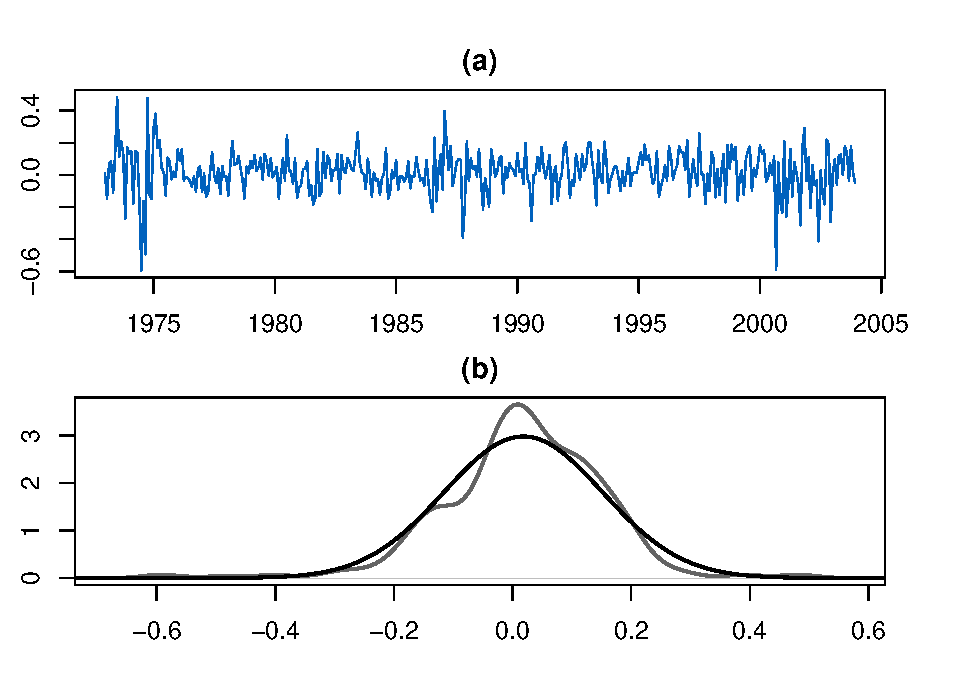
\includegraphics[width=0.85\textwidth]{ass_4_files/figure-latex/unnamed-chunk-3-1.pdf}
\end{center}

接下来拟合均值方程,作ACF、PACF图如下所示,从两幅图中都可以看出呈现拖尾的情形,因此可以选择\textbf{ARMA(1,1)}模型。

\begin{Shaded}
\begin{Highlighting}[]
\KeywordTok{par}\NormalTok{(}\DataTypeTok{mfrow =} \KeywordTok{c}\NormalTok{(}\DecValTok{2}\NormalTok{, }\DecValTok{1}\NormalTok{), }\DataTypeTok{mar =} \KeywordTok{c}\NormalTok{(}\DecValTok{4}\NormalTok{,}\DecValTok{4}\NormalTok{,}\FloatTok{0.5}\NormalTok{,}\DecValTok{1}\NormalTok{), }\DataTypeTok{oma =} \KeywordTok{c}\NormalTok{(}\DecValTok{1}\NormalTok{,}\DecValTok{1}\NormalTok{,}\DecValTok{1}\NormalTok{,}\DecValTok{2}\NormalTok{))}
\KeywordTok{acf}\NormalTok{(x, }\DataTypeTok{main =} \StringTok{""}\NormalTok{)}
\KeywordTok{pacf}\NormalTok{(x, }\DataTypeTok{main =} \StringTok{""}\NormalTok{)}
\end{Highlighting}
\end{Shaded}

\begin{center}
	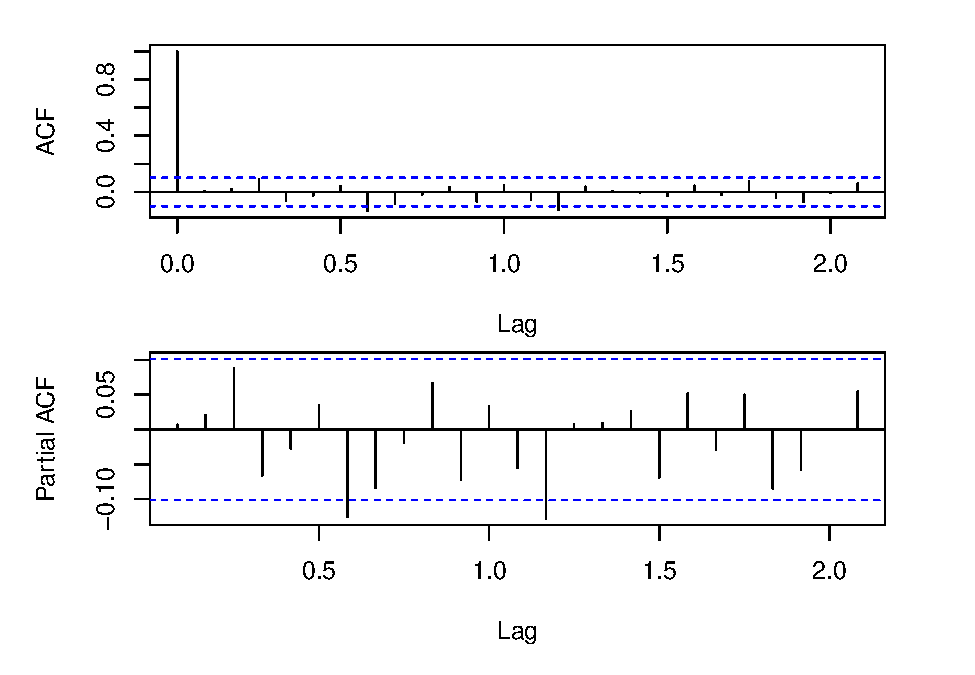
\includegraphics{ass_4_files/figure-latex/unnamed-chunk-4-1.pdf}
\end{center}

拟合\textbf{ARMA(1,1)}模型,并对残差序列进行白噪声检验,原假设\$H\_0:,\$序列为白噪声,输出对应的P值

\begin{Shaded}
\begin{Highlighting}[]
\NormalTok{x.fit <-}\StringTok{ }\KeywordTok{arima}\NormalTok{(x, }\DataTypeTok{order =} \KeywordTok{c}\NormalTok{(}\DecValTok{1}\NormalTok{, }\DecValTok{0}\NormalTok{, }\DecValTok{1}\NormalTok{))}

\KeywordTok{sapply}\NormalTok{(}\DecValTok{1}\OperatorTok{:}\DecValTok{6}\NormalTok{, }\ControlFlowTok{function}\NormalTok{(i) \{}
  \KeywordTok{Box.test}\NormalTok{(x.fit}\OperatorTok{$}\NormalTok{residual, }\DataTypeTok{type =} \StringTok{"Ljung-Box"}\NormalTok{, }\DataTypeTok{lag =}\NormalTok{ i) }\OperatorTok{$}\StringTok{ }\NormalTok{p.value}
\NormalTok{\})}
\end{Highlighting}
\end{Shaded}

\begin{verbatim}
## [1] 0.7790473 0.9449843 0.4138305 0.3314833 0.4381149 0.4789648
\end{verbatim}

可以认为\textbf{ARMA(1,1)}基本提取了序列中的自相关结构。

接下来检验对数收益率序列是否包含ARCH效应,绘制残差平方序列的ACF图和PACF图

\begin{Shaded}
\begin{Highlighting}[]
\KeywordTok{par}\NormalTok{(}\DataTypeTok{mfrow =} \KeywordTok{c}\NormalTok{(}\DecValTok{2}\NormalTok{, }\DecValTok{1}\NormalTok{), }\DataTypeTok{mar =} \KeywordTok{c}\NormalTok{(}\DecValTok{4}\NormalTok{,}\DecValTok{4}\NormalTok{,}\FloatTok{0.5}\NormalTok{,}\DecValTok{1}\NormalTok{), }\DataTypeTok{oma =} \KeywordTok{c}\NormalTok{(}\DecValTok{1}\NormalTok{,}\DecValTok{1}\NormalTok{,}\DecValTok{1}\NormalTok{,}\DecValTok{2}\NormalTok{))}
\KeywordTok{acf}\NormalTok{(x.fit}\OperatorTok{$}\NormalTok{residuals}\OperatorTok{^}\DecValTok{2}\NormalTok{, }\DataTypeTok{main =} \StringTok{""}\NormalTok{)}
\KeywordTok{pacf}\NormalTok{(x.fit}\OperatorTok{$}\NormalTok{residuals}\OperatorTok{^}\DecValTok{2}\NormalTok{, }\DataTypeTok{main =} \StringTok{""}\NormalTok{)}
\end{Highlighting}
\end{Shaded}

\begin{center}
	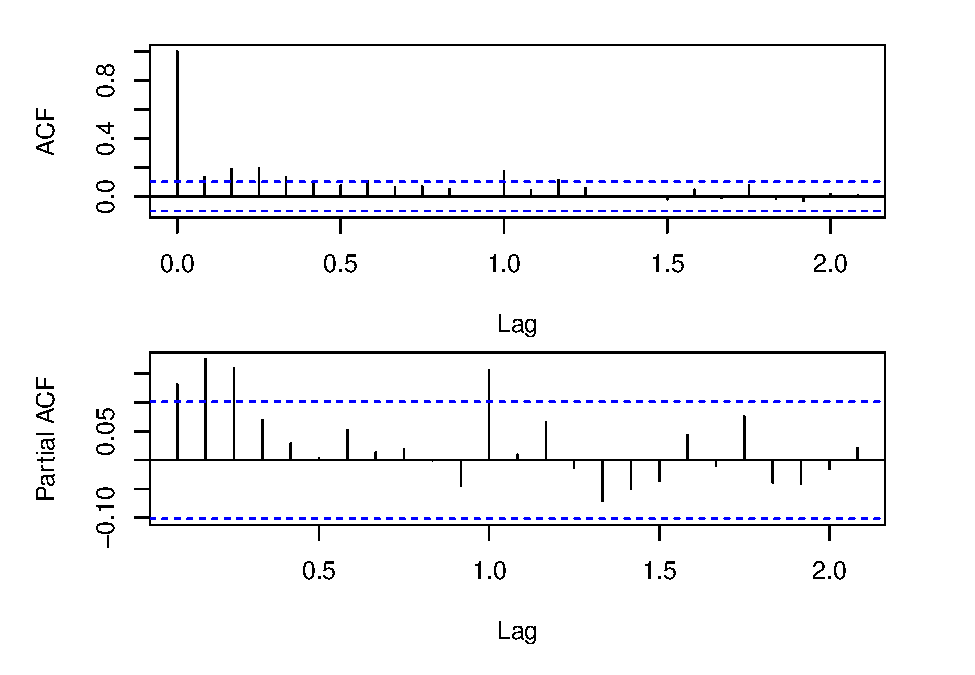
\includegraphics{ass_4_files/figure-latex/unnamed-chunk-6-1.pdf}
\end{center}

对残差平方序列进行Portmantea
Q检验,原假设\$H\_0:,\$残差平方序列纯随机,即方差齐性,P值结果如下

\begin{Shaded}
\begin{Highlighting}[]
\KeywordTok{sapply}\NormalTok{(}\DecValTok{1}\OperatorTok{:}\DecValTok{6}\NormalTok{, }\ControlFlowTok{function}\NormalTok{(i) \{}
  \KeywordTok{Box.test}\NormalTok{(x.fit}\OperatorTok{$}\NormalTok{residual}\OperatorTok{^}\DecValTok{2}\NormalTok{, }\DataTypeTok{type =} \StringTok{"Ljung-Box"}\NormalTok{, }\DataTypeTok{lag =}\NormalTok{ i) }\OperatorTok{$}\StringTok{ }\NormalTok{p.value}
\NormalTok{\})}
\end{Highlighting}
\end{Shaded}

\begin{verbatim}
## [1] 1.095670e-02 4.419376e-05 1.517263e-07 2.598256e-08 1.386019e-08
## [6] 1.699952e-08
\end{verbatim}

前六阶检验的P值都特别小,说明存在低阶的显著的自相关性,存在ARCH效应。根据ACF和PACF图的情况,将波动方程定阶为\textbf{GARCH(1,1)},结合均值方程,模型为\textbf{ARMA(1,1)+GARCH(1,1)}

\begin{Shaded}
\begin{Highlighting}[]
\KeywordTok{library}\NormalTok{(fGarch)}
\end{Highlighting}
\end{Shaded}

\begin{Shaded}
\begin{Highlighting}[]
\NormalTok{m1 <-}\StringTok{ }\KeywordTok{garchFit}\NormalTok{(intc }\OperatorTok{~}\StringTok{ }\KeywordTok{arma}\NormalTok{(}\DecValTok{1}\NormalTok{, }\DecValTok{1}\NormalTok{) }\OperatorTok{+}\StringTok{ }\KeywordTok{garch}\NormalTok{(}\DecValTok{1}\NormalTok{, }\DecValTok{1}\NormalTok{), }\DataTypeTok{data =}\NormalTok{ w, }\DataTypeTok{trace =} \OtherTok{FALSE}\NormalTok{)}
\KeywordTok{summary}\NormalTok{(m1)}
\end{Highlighting}
\end{Shaded}

\begin{verbatim}
## Coefficient(s):
##         mu         ar1         ma1       omega      alpha1       beta1  
##  0.0096245   0.4098051  -0.3832953   0.0010924   0.0808624   0.8547395  
##
## Error Analysis:
##         Estimate  Std. Error  t value Pr(>|t|)    
## mu      0.009624    0.012183    0.790  0.42952    
## ar1     0.409805    0.711036    0.576  0.56438    
## ma1    -0.383295    0.720425   -0.532  0.59470    
## omega   0.001092    0.000530    2.061  0.03928 *  
## alpha1  0.080862    0.028380    2.849  0.00438 ** 
## beta1   0.854739    0.046413   18.416  < 2e-16 ***
## ---
## Signif. codes:  0 '***' 0.001 '**' 0.01 '*' 0.05 '.' 0.1 ' ' 1
## 
## Log Likelihood:
##  239.6704    normalized:  0.6442751 
## 
## Standardised Residuals Tests:
##                                 Statistic p-Value     
##  Jarque-Bera Test   R    Chi^2  159.0297  0           
##  Shapiro-Wilk Test  R    W      0.967951  2.727838e-07
##  Ljung-Box Test     R    Q(10)  9.558936  0.4800025   
##  Ljung-Box Test     R    Q(15)  16.37201  0.3577674   
##  Ljung-Box Test     R    Q(20)  17.70885  0.606581    
##  Ljung-Box Test     R^2  Q(10)  0.5568293 0.9999889   
##  Ljung-Box Test     R^2  Q(15)  9.771177  0.8338812   
##  Ljung-Box Test     R^2  Q(20)  11.34174  0.9368743   
##  LM Arch Test       R    TR^2   8.768857  0.7225361   
## 
## Information Criterion Statistics:
##       AIC       BIC       SIC      HQIC 
## -1.256292 -1.193084 -1.256802 -1.231191
\end{verbatim}

其中ar1、ma1项的系数并不显著,说明均值方程相对整个模型波动的影响并不明显;从序列原始的ACF图也可以认为其自相关系数0阶截尾,均值方程为常数。因此将模型调整为\textbf{GARCH(1,1)}查看结果

\begin{Shaded}
\begin{Highlighting}[]
\NormalTok{m1 <-}\StringTok{ }\KeywordTok{garchFit}\NormalTok{(intc }\OperatorTok{~}\StringTok{ }\KeywordTok{garch}\NormalTok{(}\DecValTok{1}\NormalTok{, }\DecValTok{1}\NormalTok{), }\DataTypeTok{data =}\NormalTok{ w, }\DataTypeTok{trace =} \OtherTok{FALSE}\NormalTok{)}
\KeywordTok{summary}\NormalTok{(m1)}
\end{Highlighting}
\end{Shaded}

\begin{verbatim}
## Coefficient(s):
##        mu      omega     alpha1      beta1  
## 0.0163276  0.0010918  0.0802716  0.8553014  
## 
## Error Analysis:
##         Estimate  Std. Error  t value Pr(>|t|)    
## mu     0.0163276   0.0062624    2.607  0.00913 ** 
## omega  0.0010918   0.0005291    2.063  0.03907 *  
## alpha1 0.0802716   0.0281162    2.855  0.00430 ** 
## beta1  0.8553014   0.0461374   18.538  < 2e-16 ***
## ---
## Signif. codes:  0 '***' 0.001 '**' 0.01 '*' 0.05 '.' 0.1 ' ' 1
## 
## Standardised Residuals Tests:
##                                 Statistic p-Value     
##  Jarque-Bera Test   R    Chi^2  156.5138  0           
##  Shapiro-Wilk Test  R    W      0.9676933 2.471139e-07
##  Ljung-Box Test     R    Q(10)  9.805485  0.4577215   
##  Ljung-Box Test     R    Q(15)  16.54435  0.346824    
##  Ljung-Box Test     R    Q(20)  17.8005   0.6005484   
##  Ljung-Box Test     R^2  Q(10)  0.5130171 0.9999925   
##  Ljung-Box Test     R^2  Q(15)  10.24557  0.8040151   
##  Ljung-Box Test     R^2  Q(20)  11.77988  0.9234441   
##  LM Arch Test       R    TR^2   9.334459  0.6741288   
## 
## Information Criterion Statistics:
##       AIC       BIC       SIC      HQIC 
## -1.266231 -1.224092 -1.266459 -1.249496
\end{verbatim}

此时所有参数都表现为显著,并且\texttt{AIC}和\texttt{BIC}的数值也有所下降。

对残差项进行Kolmogorov-Smirnov正态性检验,原假设\$H\_0:,\$残差序列服从正态分布。

\begin{Shaded}
\begin{Highlighting}[]
\KeywordTok{ks.test}\NormalTok{(x.fit}\OperatorTok{$}\NormalTok{residuals, }
        \KeywordTok{dnorm}\NormalTok{(s2, }\DataTypeTok{mean =}\NormalTok{ stat}\OperatorTok{$}\NormalTok{mean, }\DataTypeTok{sd =}\NormalTok{ stat}\OperatorTok{$}\NormalTok{sd),}
        \DataTypeTok{alternative =} \KeywordTok{c}\NormalTok{(}\StringTok{"two.sided"}\NormalTok{, }\StringTok{"less"}\NormalTok{, }\StringTok{"greater"}\NormalTok{),}
        \DataTypeTok{exact =} \OtherTok{NULL}\NormalTok{)}
\end{Highlighting}
\end{Shaded}

\begin{verbatim}
## 
##  Two-sample Kolmogorov-Smirnov test
## 
## data:  x.fit$residuals and dnorm(s2, mean = stat$mean, sd = stat$sd)
## D = 0.49194, p-value < 2.2e-16
## alternative hypothesis: two-sided
\end{verbatim}

P值几乎接近0,因此误差项分布显著异于正态分布,设定为t分布重新拟合模型

\begin{Shaded}
\begin{Highlighting}[]
\NormalTok{m1 <-}\StringTok{ }\KeywordTok{garchFit}\NormalTok{(intc }\OperatorTok{~}\StringTok{ }\KeywordTok{garch}\NormalTok{(}\DecValTok{1}\NormalTok{, }\DecValTok{1}\NormalTok{), }\DataTypeTok{data =}\NormalTok{ w,}
               \DataTypeTok{cond.dist =} \StringTok{"std"}\NormalTok{, }\DataTypeTok{trace =} \OtherTok{FALSE}\NormalTok{)}
\KeywordTok{summary}\NormalTok{(m1)}
\end{Highlighting}
\end{Shaded}

\begin{verbatim}
## Coefficient(s):
##        mu      omega     alpha1      beta1      shape  
## 0.0219121  0.0014771  0.1036656  0.8085661  6.6892311  
## 
## Std. Errors:
##  based on Hessian 
## 
## Error Analysis:
##         Estimate  Std. Error  t value Pr(>|t|)    
## mu     0.0219121   0.0059313    3.694 0.000220 ***
## omega  0.0014771   0.0007917    1.866 0.062064 .  
## alpha1 0.1036656   0.0408173    2.540 0.011093 *  
## beta1  0.8085661   0.0685649   11.793  < 2e-16 ***
## shape  6.6892311   1.9602897    3.412 0.000644 ***
## ---
## Signif. codes:  0 '***' 0.001 '**' 0.01 '*' 0.05 '.' 0.1 ' ' 1
## 
## Log Likelihood:
##  251.7896    normalized:  0.6768539 
## 
## Standardised Residuals Tests:
##                                 Statistic p-Value     
##  Jarque-Bera Test   R    Chi^2  184.8699  0           
##  Shapiro-Wilk Test  R    W      0.9647736 8.306688e-08
##  Ljung-Box Test     R    Q(10)  9.545124  0.4812646   
##  Ljung-Box Test     R    Q(15)  16.54094  0.3470391   
##  Ljung-Box Test     R    Q(20)  17.98089  0.5886671   
##  Ljung-Box Test     R^2  Q(10)  0.6650225 0.9999743   
##  Ljung-Box Test     R^2  Q(15)  10.71018  0.7728558   
##  Ljung-Box Test     R^2  Q(20)  12.09555  0.912748    
##  LM Arch Test       R    TR^2   9.870077  0.6273576   
## 
## Information Criterion Statistics:
##       AIC       BIC       SIC      HQIC 
## -1.326826 -1.274153 -1.327181 -1.305908
\end{verbatim}

至此模型\texttt{AIC}和\texttt{BIC}的结果最小,模型效果达到相对最优。最后的模型为
\[
x_t = 0.02191+\varepsilon_t,\quad
\sigma^2_t = 0.00148+0.1037\varepsilon_{t-1}+0.8086\sigma_{t-1}^2
\] 进行向前五步预测

\begin{Shaded}
\begin{Highlighting}[]
\NormalTok{pre <-}\StringTok{ }\KeywordTok{predict}\NormalTok{(m1, }\DecValTok{5}\NormalTok{)}
\NormalTok{pre}
\end{Highlighting}
\end{Shaded}

\begin{verbatim}
##   meanForecast meanError standardDeviation
## 1   0.02191214 0.1194190         0.1194190
## 2   0.02191214 0.1203592         0.1203592
## 3   0.02191214 0.1212105         0.1212105
## 4   0.02191214 0.1219819         0.1219819
## 5   0.02191214 0.1226813         0.1226813
\end{verbatim}

\end{document}
